\documentclass[a4paper,12pt]{report}

\usepackage{pdfpages}
\usepackage[utf8]{inputenc}
\usepackage[catalan]{babel}
\usepackage{amsmath}
\usepackage{graphicx}
\usepackage{hyperref}
\usepackage{booktabs}
\usepackage[sorting=none]{biblatex}
\usepackage{float}
\usepackage{verbatim}
\usepackage{geometry}
\usepackage{pdflscape}

\addbibresource{biblio.bib}

\title{DISSENY I ANÀLISI DE TÈCNIQUES DE
CLUSTERING APLICADES A SISTEMES DE
RECOMANACIÓ}
\author{POL FONOYET GONZÁLEZ}
\date{\today}

\begin{document}


\setcounter{secnumdepth}{4}  % Assegurar-se que es numeren fins a subsubsecció

\setlength{\parskip}{10pt}

\begin{titlepage}
    
    % imatge de la UPC
    \vspace*{-3cm}
    \hspace{-0.15\textwidth}
    
\includegraphics[width=0.15\textwidth]{Figuras/logoUPC.png}
    \hspace{0.02\textwidth}
    
\includegraphics[width=1\textwidth]{Figuras/logoFIB.png}\par

    % título en negrita
    \vspace{3cm}
    \centering
    \Large\textbf{DISSENY I ANÀLISI DE TÈCNIQUES DE CLUSTERING APLICADES A SISTEMES DE RECOMANACIÓ}

    % nombre del autor
    \vspace{2cm}
    \centering
    \large\textbf{POL FONOYET GONZÁLEZ}\\
    \vspace{0.5cm}
    \textbf{Treball Final de Grau}\\
    \textbf{Lliurable 4: Document final}\\
    \vspace{0.5cm}
    \Large 19 de març de 2025

    % información de la universidad
    \vspace{2cm}
    \centering
    \small
    \textbf{Director/a}\\
    CONRADO MARTÍNEZ PARRA (Departament de Ciències de la Computació)\\
    \vspace{0.5cm}
    \textbf{Titulació}\\
    Grau en Enginyeria Informàtica (Computació)\\
    \vspace{0.5cm}
    \textbf{Tutor GEP}\\
    Olga Pons Peregort\\
    \vspace{0.5cm}
    \textbf{Facultat d'Informàtica de Barcelona (FIB)}\\
    \vspace{0.5cm}
    \textbf{Universitat Politècnica de Catalunya (UPC) - BarcelonaTech}\\


\end{titlepage}

\newgeometry{top=2.5cm, left=3cm, right=2.5cm, bottom=2.5cm} % Ajustar el marge superior després de la portada

\tableofcontents

\listoffigures

\listoftables

\chapter{Contextualització i Abast del projecte}

\section{Introducció}

Aquest treball de final de grau s'ha dut a terme en el Grau d'Enginyeria Informàtica impartit en el marc de la Facultat d'Informàtica de Barcelona (FIB), pertanyent a la Universitat Politècnica de Catalunya (UPC). Dins d'aquest programa acadèmic, s'ofereixen diverses àrees d'especialització, entre les quals destaca la de Computació. El present projecte se situa en aquesta especialització, centrant el seu enfocament en temàtiques clau com la Intel·ligència Artificial (IA) i l'Aprenentatge Automàtic (AA).

\subsection{Context}

A mesura que la quantitat de dades generades en l'entorn digital segueix augmentant, la necessitat de tècniques avançades per analitzar i processar aquesta informació es torna cada vegada més crítica.
En aquest escenari, els sistemes de recomanació han emergit com a eines essencials per personalitzar l'experiència d'usuari, filtrant i suggerint continguts rellevants en funció de les seves preferències i comportaments \cite{Idrees_2024}.
Aquests sistemes exerceixen un paper fonamental en àmbits tan diversos com el comerç electrònic, l'entreteniment i l'educació, permetent millorar la interacció i satisfacció dels usuaris \cite{Kantor_Ricci_Rokach_Shapira_2011}.
Segons un informe de McKinsey, el 35\% del que els consumidors compren a Amazon i el 75\% del que veuen a Netflix provenen de recomanacions \cite{MacKenzie_Meyer_Noble_2013}.

La personalització efectiva requereix comprendre les preferències i comportaments dels usuaris.
El filtratge col·laboratiu, una tècnica àmpliament utilitzada, enfronta dos grans desafiaments: l'escalabilitat i la dispersió.
A mesura que augmenta la quantitat d'usuaris i ítems, les matrius d'utilitat es tornen enormes, cosa que incrementa el cost computacional \cite{sarwar2001item}.
A més, la majoria dels usuaris interactuen amb només una fracció dels ítems, resultant en matrius molt disperses, cosa que dificulta el càlcul precís de similituds \cite{adomavicius2005toward}.

Les tècniques de clustering, com k-means, DBSCAN i k-NN, permeten agrupar usuaris amb interessos similars, facilitant la identificació de patrons i la generació de recomanacions més precises \cite{jain2008data}.
En aplicar clustering com a pas previ al filtratge col·laboratiu, es poden crear grups més petits i homogènics, reduint la complexitat de les matrius i el temps de còmput.
A més, en treballar amb grups d'usuaris similars, es redueix el problema de la dispersió, ja que els usuaris dins d'un mateix clúster tendeixen a tenir més interaccions en comú \cite{Kantor_Ricci_Rokach_Shapira_2011}.

Aquest projecte se centra en el disseny i l'anàlisi de tècniques de clustering aplicades a sistemes de recomanació, amb l'objectiu d'optimitzar la qualitat i el rendiment de les recomanacions.

\subsection{Conceptes}

A continuació, es defineixen els termes i conceptes clau relacionats amb el tema d'estudi.

\subsubsection{Sistema de Recomanació}

Un sistema de recomanació és un sistema que calcula i proporciona contingut rellevant a l'usuari basant-se en el coneixement de l'usuari, el contingut i les interaccions entre l'usuari i l'element. \cite{falk2019practical}

El propòsit d’una plataforma de recomanació de contingut és facilitar als usuaris l’accés a informació rellevant de manera ràpida i eficient, millorant la seva experiència i fomentant la seva permanència en el servei. Al mateix temps, busca optimitzar recursos i maximitzar beneficis per al proveïdor, assegurant que el contingut ofert sigui atractiu i sostenible econòmicament. Això es fa mitjançant sistemes intel·ligents que analitzen el comportament dels usuaris per oferir opcions personalitzades, tot mantenint un equilibri entre satisfacció i rendibilitat.

\subsubsection{Filtratge Col·laboratiu}

La idea principal dels enfocaments de recomanació col·laborativa és aprofitar la informació sobre el comportament passat o les opinions d'una comunitat d'usuaris existent per predir quins elements li agradaran o interessaran més a l'usuari actual del sistema \cite{Jannach2011}.

\begin{figure}[h]
    \centering
    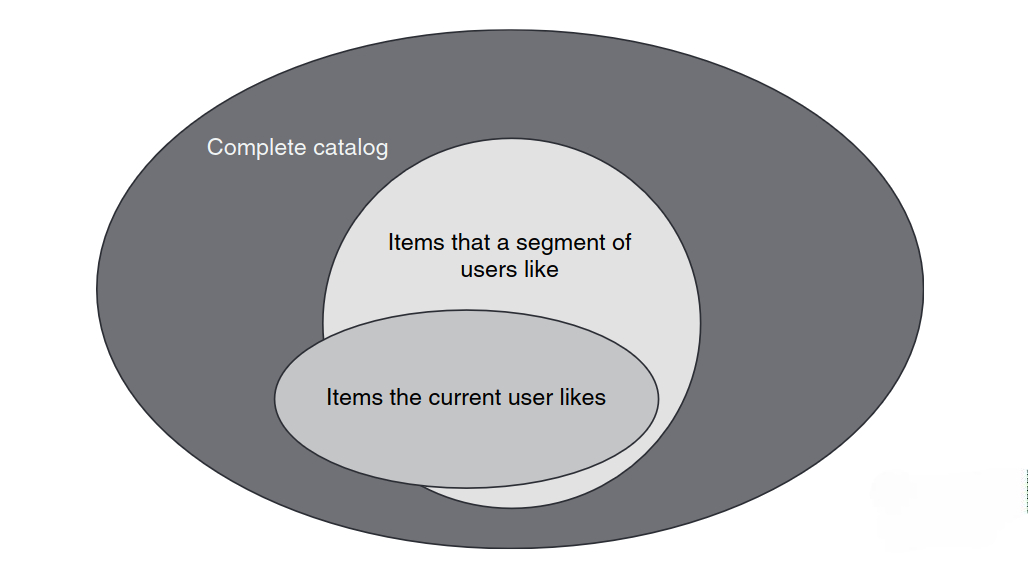
\includegraphics[width=0.8\textwidth]{Figuras/DiagramaFiltratgeCol.jpg}
    \caption{Diagrama de filtratge col·laboratiu \cite{falk2019practical}}
    \label{fig:collaborative-filtering-diagram}
\end{figure}

La figura \ref{fig:collaborative-filtering-diagram} il·lustra com funciona el filtrat col·laboratiu. El cercle exterior representa el catàleg complet. El cercle intermedi representa un grup d'usuaris que han consumit elements similars. El sistema de recomanació suggereix elements del cercle més proper (davant), partint de la idea que si aquests usuaris coincideixen en preferències amb l’usuari actual, aquest també preferirà els elements que han consumit.

El grup es determina mitjançant la superposició entre els elements que han agradat als usuaris i els que ha agradat a l’usuari actual. Les recomanacions corresponen a la part del cercle intermedi no coberta pel cercle de l’usuari actual (és a dir, els elements que ell/ella no ha consumit però sí el grup semblant).


\subsubsection{Clustering}

El clustering, segons la perspectiva de \cite{jain2008data}, es concep fonamentalment com l'organització de dades dins de grups cohesionats, on la semblança entre els elements d'un mateix grup supera la que mantenen amb els d'altres grups.
Aquesta tècnica, que es fonamenta en mesures de similitud o distància, és clau en l’anàlisi de dades sense supervisió, ja que permet identificar estructures o patrons latents en els conjunts de dades sense necessitat d’etiquetes prèvies. Així, el clustering facilita la comprensió i la interpretació de grans volums d’informació, sent una eina fonamental tant en l’exploració de dades com en l’aprenentatge automàtic. 

\subsection{Identificació del problema}

En aquest treball es desenvoluparà una comparativa entre diferents tècniques de clustering aplicades als sistemes de recomanació. El problema es pot dividir en tres blocs de treball:

\subsubsection{Selecció i tractament del conjunt de dades}

Aquest primer bloc consisteix en la recerca, selecció i/o creació de datasets, tant reals com sintètics, que representin diferents volums de dades i nivells de dispersió,  
assegurant que els escenaris simulats reflecteixin les diverses situacions que es poden presentar en entorns reals.

\subsubsection{Desenvolupament del sistema de recomanació}

En aquest segon bloc es construirà el sistema de recomanació, on el clustering actuarà com a pas previ al filtratge col·laboratiu.  
Aquest també capturarà diferents mètriques de precisió i eficiència computacional.  
A més, estarà dissenyat de manera que es pugui escollir amb quina tècnica de clusterització ha de funcionar.

\subsubsection{Comparació de resultats i anàlisi del rendiment}

Finalment, es compararan els resultats de les diferents tècniques emprades amb els diferents datasets amb l'objectiu de determinar quina tècnica ofereix el millor equilibri entre eficàcia i eficiència en diferents escenaris.

\subsection{Actors implicats}

En aquest projecte hi ha diversos actors implicats:

\begin{itemize}
    \item \textbf{Estudiant/investigador}: Responsable de desenvolupar, implementar i analitzar les tècniques de clustering aplicades als sistemes de recomanació.
    \item \textbf{Director/tutor acadèmic}: Responsable de supervisar el progrés del projecte i oferir orientació acadèmica.
    \item \textbf{Comunitat acadèmica}: Inclou altres estudiants, investigadors i professionals interessats en els resultats del projecte. Els principals beneficiaris dels resultats serien els investigadors en temes de sistemes de recomanació i aprenentatge automàtic.
    \item \textbf{Proveïdors de datasets}: Organitzacions o comunitats que proporcionen conjunts de dades reals i sintètics per a l'entrenament i proves dels algorismes de clustering.
\end{itemize}

\section{Justificació}

L'augment exponencial de la informació digital ha generat un repte important per als sistemes de recomanació, ja que els mètodes tradicionals, com el filtratge col·laboratiu, es veuen limitats per problemes d'escala i dispersió de dades.
Aquesta situació posa de manifest la necessitat d'explorar noves estratègies per millorar tant la precisió com l'eficiència en la generació de recomanacions.

En aquest context, l'aplicació de tècniques de clustering com a pas previ ofereix un potencial significatiu: agrupar usuaris i ítems en clústers més cohesius redueix la dimensió de la matriu usuari-ítem, minimitza el cost computacional i afavoreix una major densitat en les dades per a càlculs més precisos.
Tot i que existeixen diverses solucions informàtiques que integren el clustering en sistemes de recomanació, en la revisió de la literatura no s'han trobat estudis que comparin explícitament els diferents algoritmes de clustering en aquest context de manera sistemàtica.

\subsection{Estat de l'art}

En els darrers anys, l'interès per optimitzar els sistemes de recomanació ha condüït a l'aplicació de diverses tècniques d'aprenentatge automàtic, amb especial èmfasi en el filtratge col·laboratiu.
Paral·lelament, s'ha observat una creixent utilització de tècniques de clustering per reduir la dimensionalitat de la matriu usuari-ítem i millorar la densitat de les dades, aspecte clau per a l'eficiència computacional i la precisió de les recomanacions.

Diversos estudis han abordat l'ús d'algoritmes com k-means i DBSCAN, entre d'altres, per agrupar usuaris amb interessos similars, facilitant així la generació de recomanacions personalitzades.
Aquestes investigacions han demostrat que el pre-processament de les dades mitjançant clustering pot reduir significativament el temps de càlcul i millorar els resultats en entorns amb grans volums de dades.

No obstant això, en la revisió de la literatura existent s'ha constatat la manca d'estudis que realitzin una comparativa explícita i sistemàtica dels diferents algoritmes de clustering aplicats específicament en el context dels sistemes de recomanació.
La major part dels treballs se centra en la implementació d'un sol mètode o en l'aplicació general del clustering sense aprofundir en la comparació directa dels resultats obtinguts per cadascun d'ells.

Aquest buit en la recerca representa una oportunitat per aportar una anàlisi més detallada i una valoració crítica dels avantatges i inconvenients de cada tècnica.
El present projecte pretén omplir aquesta llacuna aportant una comparativa exhaustiva dels principals algoritmes de clustering, la qual cosa servirà com a referència tant per a la comunitat acadèmica com per a la indústria, i contribuirà a la millora dels sistemes de recomanació en entorns reals.

\subsection{Selecció d'eines}

En aquest projecte s'ha realitzat una acurada elecció de les eines i entorns de treball, tenint en compte la necessitat d'executar càlculs numèrics, processar grans volums de dades, implementar tècniques d'aprenentatge automàtic i visualitzar els resultats d'una manera clara i professional.

\textbf{Python} és el llenguatge de programació seleccionat per la seva sintaxi senzilla, la seva versatilitat i la seva àmplia comunitat, que garanteix un suport continu i una gran quantitat de recursos per al desenvolupament d'aplicacions científiques i d'aprenentatge automàtic.

Per al processament de dades i càlculs numèrics, s'empren les llibreries \textbf{NumPy} i \textbf{Pandas}. NumPy facilita la manipulació d'arrays i l'execució d'operacions matemàtiques d'alt rendiment, mentre que Pandas proporciona estructures de dades eficients (com els DataFrames) per a la manipulació i anàlisi de dades, essent essencials per a la preparació i neteja dels datasets.

La implementació i comparativa dels diferents algoritmes de clustering es realitzarà amb la llibreria \textbf{Scikit-learn}, que inclou una àmplia varietat d'eines per a l'aprenentatge automàtic, incloent mètodes de classificació, regressió, clustering i reducció de dimensionalitat. Aquesta eina és fonamental per a dur a terme experiments rigorosos i comparatius.

Per a la visualització dels resultats i l'anàlisi exploratòria, s'utilitzarà \textbf{Matplotlib}, que permet generar gràfics i representacions visuals personalitzables i de gran qualitat, facilitant així la interpretació de les dades.

A més, s'incorpora el paquet \textbf{Surprise}, especialitzat en sistemes de recomanació, que facilita la implementació de tècniques de filtratge col·laboratiu i la comparativa amb els mètodes basats en clustering.

Pel que fa als entorns de desenvolupament, s'ha optat per \textbf{Jupyter Notebook}, que permet combinar codi, visualitzacions i documentació en un entorn interactiu, afavorint la iteració i validació ràpida de hipòtesis.
El control de versions es gestionarà amb \textbf{Git}, assegurant un seguiment acurat dels canvis.
Finalment, \textbf{LaTeX} s'utilitzarà per a la redacció i formatatge del document final, garantint una presentació clara, estructurada i professional dels resultats.

\section{Abast}

\subsection{Objectius}

L'objectiu principal d'aquest projecte és desenvolupar i comparar diferents tècniques de clustering en el context dels sistemes de recomanació. Això implica: 

\begin{itemize} 
    \item Implementar un mòdul de clustering basat en tècniques particionals clàssiques. 
    \item Desenvolupar versions alternatives que utilitzin tècniques com clustering difús i jeràrquic. 
    \item Analitzar i comprendre el funcionament i les particularitats de cada mètode de clustering. 
    \item Avaluar, mitjançant mètriques específiques, la precisió, l'eficiència computacional i la robustesa de cada enfocament. 
    \item Contribuir al coneixement en l'àmbit dels sistemes de recomanació, aportant una comparativa rigorosa i documentada que pugui servir de referència tant per a la comunitat acadèmica com per a futurs desenvolupaments en l'àrea. 
\end{itemize}

\subsection{Subobjectius}

Per assolir l'objectiu principal es plantegen els següents subobjectius: 

\begin{itemize} 
    \item Dur a terme una revisió bibliogràfica exhaustiva sobre tècniques de clustering i la seva aplicació en sistemes de recomanació. 
    \item Dissenyar una arquitectura modular que permeti integrar fàcilment diferents algoritmes de clustering en el sistema de recomanació. 
    \item Implementar els algorismes seleccionats de manera que es puguin comparar de forma sistemàtica. 
    \item Capturar i analitzar mètriques clau, com ara el temps d'execució, la densitat de dades i la precisió de les recomanacions. 
    \item Elaborar una documentació detallada que reculli els resultats experimentals i les conclusions obtingudes. 
\end{itemize}

\subsection{Requeriments}

\subsubsection{Funcionals}

\begin{itemize} 
    \item \textbf{Recollida i tractament de dades:} Seleccionar conjunts de dades (reals o sintètics) que representin diferents escenaris en sistemes de recomanació.
    Aplicar tècniques de preprocessament i neteja per garantir la qualitat de les dades per a l'anàlisi.
    \item \textbf{Implementació dels algorismes de clustering:} Desenvolupar implementacions de diferents tècniques de clustering (particional clàssic, difús i jeràrquic).
    Adaptar els algorismes per estudiar el seu comportament i comparativa en diferents contextos.
    \item \textbf{Anàlisi dels resultats:} Definir i aplicar mètriques d'avaluació que permetin comparar de manera rigorosa els diferents mètodes.
    Interpretar els resultats per identificar avantatges, limitacions i possibles àrees de millora de cada tècnica.
\end{itemize}

\subsubsection{No funcionals}

\begin{itemize} 
    \item \textbf{Claredat i documentació:} Redactar una documentació completa i exhaustiva que reculli la metodologia, els procediments experimentals i l'anàlisi dels resultats.
    \item \textbf{Reproductibilitat:} Assegurar que els experiments es puguin reproduir seguint la metodologia descrita, facilitant la verificació i validació dels resultats.
    \item \textbf{Validesa dels resultats:} Garantir que les tècniques aplicades permetin arribar a conclusions rigoroses i ben fonamentades, centrant-se en l'anàlisi comparativa més que en la implementació de solucions optimitzades.
\end{itemize}

\subsection{Obstacles i riscos}

\subsubsection{Obstacles}

Els principals obstacles que es poden trobar en el desenvolupament del projecte són:

\begin{itemize}
    \item \textbf{Falta de coneixement profund en la matèria:} L'autor del treball no té un gran coneixement previ de les diferents tècniques de clustering ni de sistemes de recomanació. Menys de la seva aplicació conjunta.
    \item \textbf{Potència computacional limitada:} El processament i anàlisi de grans volums de dades poden requerir recursos computacionals elevats.
    \item \textbf{Documentació extensa:} La normativa actual dels TFG exigeix la generació d’una àmplia documentació, incloent-hi entregables de GEP i la memòria. Tot i que la seva elaboració demanda una inversió de temps considerable, aquests materials permeten demostrar que s’han aplicat correctament les competències adquirides durant la titulació.
\end{itemize}

\subsubsection{Riscos}

Els riscos associats al projecte inclouen: 

\begin{itemize}
    \item \textbf{Elements imprevistos en el desenvolupament:} Dificultats tècniques o situacions no anticipades poden afectar el progrés del projecte.
    \item  \textbf{Gestió del temps:} La coordinació entre la implementació, els experiments i la redacció de la documentació pot resultar més complexa del previst. L'autor també està cursant assignatures que podrien demandar pics d'activitat inesperats.
    \item \textbf{Accidents o imprevistos personals:} Eventualitats que afectin la disponibilitat de temps per al desenvolupament del projecte.
\end{itemize}

\section{Metodologia i rigor}

L'èxit de qualsevol projecte depèn en gran mesura de la implementació de mètodes estructurats i rigorosos, que estableixen un marc organitzat per afavorir l'eficiència, la qualitat i una comunicació efectiva.

\subsection{Metodologia de treball}

Atès que és un projecte individual, una metodologia àgil i flexible com Kanban és ideal. El mètode Kanban és una metodologia àgil que es fonamenta en la visualització del projecte per millorar la transparència i la col·laboració entre els membres de l'equip.
Va ser creat per Taiichi Ohno als anys 40 per a la gestió de la producció, però es va adaptar al món de la gestió de projectes.
Es distingeix per la seva simplicitat i per la seva capacitat d’adaptar-se a organitzacions amb estructures jeràrquiques tradicionals.
Kanban funciona amb un sistema visual que permet fer un seguiment clar del progrés del projecte \cite{Person_2025}.

\begin{figure}[H]
    \centering
    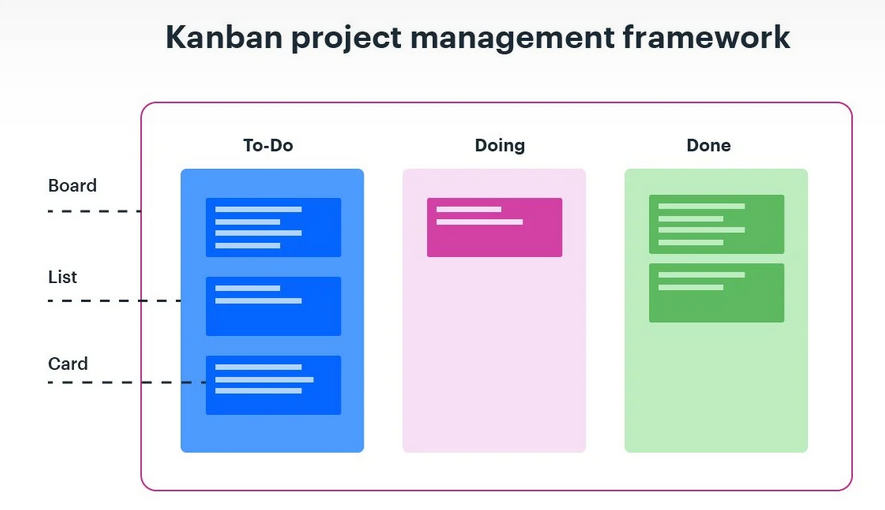
\includegraphics[width=0.8\textwidth]{Figuras/KANBAN.png}
    \caption{Diagrama il·lustratiu del flux de treball segons la metodologia Kanban \cite{Person_2025}}
    \label{fig:kanban}
\end{figure}

A la figura \ref{fig:kanban} es mostren tres columnes principals: \textit{To Do} (Per fer), \textit{Doing} (En procés) i \textit{Done} (Fet).
Aquestes columnes representen les fases de treball en què es troben les tasques. Els membres de l'equip traslladen les tasques des de la columna de \textit{To Do} cap a \textit{In Progress} quan comencen a treballar-hi i, finalment, a \textit{Done} quan s’acaben, seguint els límits de treball en curs (WIP) per garantir que el flux de treball es mantingui eficaç.

\begin{figure} [H]
    \centering
    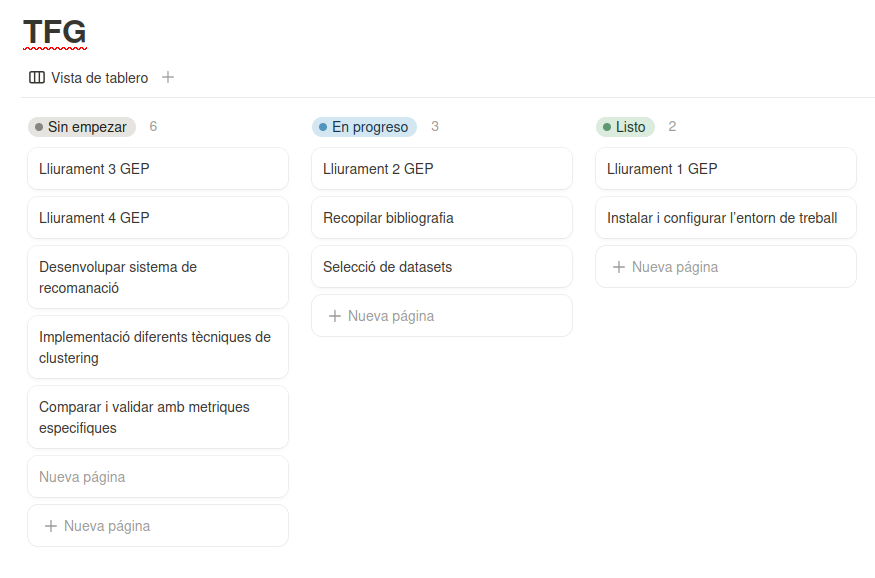
\includegraphics[width=0.8\textwidth]{Figuras/Notion.png}
    \caption{Captura de pantalla de la plataforma Notion}
    \label{fig:notion}
\end{figure}

Per a la implementació d'aquesta metodologia s'utilitzarà la web de Notion.
Notion és una plataforma col·laborativa i de gestió de projectes que facilita l'organització de tasques de manera visual i flexible.
Com es veu a la figura \ref{fig:notion}, permet dividir les tasques en els tres grups esmentats, cosa que s'alinea perfectament amb l'enfocament Kanban, assegurant una gestió eficient, una comunicació fluida i una transparència en el seguiment del progrés del projecte.

\subsection{Seguiment}

Per tal de verificar que el desenvolupament del projecte s’ajusta als requeriments establerts i per corregir sense dilació qualsevol desviació que pugui sorgir, es realitzarà el seguiment del projecte mitjançant reunions presencials cada dues setmanes. En aquestes trobades es procedirà a:

\begin{itemize}
    \item \textbf{Analitzar el progrés global:} Revisarem l’evolució tant del programari com de la documentació, identificant els avanços assolits i les possibles àrees de millora.
    \item \textbf{Detectar dificultats i incidències:} S'exposaran les dificultats trobades durant el desenvolupament, així com qualsevol desviació respecte als requisits inicials.
    \item \textbf{Establir mesures correctores:} Es discutiran i acordaran les millores i ajustaments necessaris per garantir l'alineació amb els objectius del projecte.
    \item \textbf{Comprovar el compliment dels requisits:} Amb l’ajuda d’indicadors clars, es verificarà el grau de compliment dels requisits i subrequisits, facilitant així una gestió proactiva de les incidències.
\end{itemize}

Aquest sistema de seguiment, basat en reunions presencials periòdiques, permetrà una presa de decisions àgil i una coordinació efectiva entre els actors implicats, assegurant que el projecte es desenvolupi de manera coherent i amb el nivell de qualitat desitjat.

\chapter{Planificació temporal}

En aquesta secció es realitzarà una planificació temporal del projecte definint tasques específiques i blocs de tasques, per tal d'obtenir una estimació realista de la seva durada.
El treball s'inicia el 27 de gener i la presentació està prevista per al 25 de juny, de manera que aquesta seria la data màxima de finalització.

El projecte es desenvoluparà durant aproximadament 140 dies, amb una durada estimada de 450 hores, equivalent als 18 crèdits ECTS que conformen el treball.
Aquesta quantitat d'hores es té en compte per calcular el temps que s'ha de dedicar a cada activitat, tal com es mostra a la Taula \ref{tab:tasques}.
La dedicació diària de dilluns a divendres serà aproximadament de 3-4 hores, i els caps de setmana es podrà dedicar més temps.
Es disposarà d'una gran flexibilitat ja que el projecte es realitza íntegrament des de casa.
Aquestes hores es podran destinar tant a la documentació com a la programació segons la necessitat.

\section{Descripció de les tasques}

En aquesta secció es descriuran totes les tasques que conformen el projecte.
Les tasques més grans es dividiran en subtasques per facilitar la comprensió de les diferents fases.
Finalment, es presentarà una taula resum de totes les activitats amb la seva descripció, durada, dependències, recursos i rols assignats, així com el diagrama de Gantt.

\subsection{GP - Gestió del Projecte}

Una gestió eficient és essencial per assegurar-ne l’èxit.
Aquesta proporciona un marc estructurat que facilita l’assoliment dels objectius de manera organitzada, dins dels límits establerts de temps, recursos i pressupost.
A més, una bona gestió permet minimitzar riscos, garantir la qualitat i adaptar-se a possibles imprevistos.
La duració total estimada per a la gestió del projecte és de \textbf{65 hores}. Aquest apartat es divideix en diverses fases clau, que es detallen a continuació.

\begin{itemize}
    \item \textbf{GP1 - Contextualització i Abast del projecte}
    
    Una bona definició de l’abast del projecte és fonamental per garantir-ne l’èxit.
    En aquesta fase inicial es determinen els objectius, els requisits, les possibles dificultats i els riscos associats.
    A més, cal haver recopilat informació prèvia sobre les tecnologies i metodologies que es volen aplicar.
    Es calcula que aquesta tasca requerirà aproximadament \textbf{15 hores}.

    \item \textbf{GP2 - Planificació temporal}
    
    Per tal de garantir una execució òptima, cal establir una planificació temporal adequada, identificant les tasques específiques, assignant responsabilitats i establint terminis clars.
    Això permet una millor organització del treball, minimitzant possibles retards i optimitzant els recursos.
    Es calcula que aquesta tasca requerirà aproximadament \textbf{15 hores}.

    \item \textbf{GP3 - Gestió Econòmica i sostenibilitat}
    
    Es durà a terme una anàlisi detallada dels costos associats al projecte, incloent tant les despeses de personal com els materials necessaris.
    A més, es tindran en compte possibles imprevistos i costos indirectes.
    També es realitzarà un informe sobre l’impacte ambiental, social i econòmic del projecte per assegurar-ne la sostenibilitat.
    En total, es preveu una dedicació de \textbf{15 hores} per aquesta tasca.

    \item \textbf{GP4 - Seguiment del projecte}
    
    El seguiment del projecte és essencial per garantir que es compleixen els objectius i els terminis establerts.
    Es realitzaran reunions quinzenals amb el supervisor per revisar l’evolució del projecte, resoldre possibles problemes i ajustar la planificació si cal.
    Aquestes trobades també permetran rebre orientació i millorar la presa de decisions.
    S’estima que es destinaran \textbf{20 hores} a aquesta fase.
\end{itemize}

\subsection{TP - Treball Previ}

El Treball Previ constitueix la base teòrica i tècnica del projecte.
Aquesta fase s’articula en tres parts fonamentals:

\begin{itemize}
    \item \textbf{TP1 - Estudi sobre sistemes de recomanació}
    
    Es realitzarà una revisió exhaustiva de la literatura existent per comprendre els principis bàsics, les metodologies actuals i les tendències en el desenvolupament de sistemes de recomanació.
    Aquesta anàlisi permetrà identificar els punts forts i les limitacions dels enfocaments tradicionals.
    Es calcula que aquesta tasca requerirà aproximadament \textbf{25 hores}.

    \item \textbf{TP2 - Estudi sobre clustering en sistemes de recomanació}
    
    S’analitzaran les diferents tècniques de clustering aplicades en entorns de recomanació, valorant com la seva implementació pot millorar la densitat de dades i reduir la complexitat computacional.
    L’objectiu és entendre l’impacte d’aquestes tècniques en la precisió i eficiència del sistema.
    Es calcula que aquesta tasca requerirà aproximadament \textbf{25 hores}.

    \item \textbf{TP3 - Preparació de l'entorn de treball}

    Consistirà en la configuració i comprovació de totes les eines i llibreries necessàries (com Python, Jupyter Notebook, Git, LaTeX, etc.) per assegurar que el desenvolupament posterior es realitzi en un entorn òptim i estable.
    Es calcula que aquesta tasca requerirà aproximadament \textbf{5 hores}.
\end{itemize}

\subsection{SD - Selecció i tractament del conjunt de dades}

Aquest apartat es centra en la gestió dels conjunts de dades que serviran de base per als experiments:

\begin{itemize}
    \item \textbf{SD1 - Recol·lecció de datasets}
    
    S’identificaran i obtindran conjunts de dades reals que representin diversos escenaris en sistemes de recomanació, tenint en compte diferents volums i nivells de dispersió.
    Aquesta tasca és clau per garantir que els experiments reflecteixin situacions reals.
    Es calcula que aquesta tasca requerirà aproximadament \textbf{15 hores}.

    \item \textbf{SD2 - Creació de datasets sintètics}
    
    Paral·lelament, es generaran conjunts de dades sintètics que permetin simular escenaris específics.
    D’aquesta manera, es podran avaluar els algorismes en entorns controlats, facilitant la comparació dels resultats i l’anàlisi dels comportaments davant diferents configuracions.
    Es calcula que aquesta tasca requerirà aproximadament \textbf{25 hores}.
\end{itemize}

\subsection{SR - Desenvolupament del sistema de recomanació}

En aquesta fase es durà a terme la implementació del sistema de recomanació mitjançant diferents mètodes de clustering.
Aquesta etapa constitueix el nucli del projecte, ja que el correcte desenvolupament de les tècniques determinarà la qualitat dels resultats obtinguts.

A cada mètode se li assignarà un temps estimat de desenvolupament segons la seva complexitat i la necessitat d'ajustament de paràmetres.
Es seguirà un esquema comú per a totes les implementacions, per garantir la comparabilitat dels resultats i la coherència en el codi.

\begin{itemize}
    \item \textbf{SR1 - Implementació amb clustering dur}
    
    Aquesta fase consistirà en la implementació amb clustering dur amb un algoritme com K-Means, un mètode de clustering dur on cada element es classifica de manera exclusiva en un clúster.
    Es realitzarà una anàlisi prèvia per determinar el nombre òptim de clústers utilitzant mètriques com l'Elbow Method o la Silhouette Score.
    Tindrà una duració estimada de \textbf{30 hores}.

    \item \textbf{SR2 - Implementació amb clustering difús}
    
    Es desenvoluparà la implementació amb clustering difús amb un mètode com Fuzzy C-Means, que permet una assignació parcial d'un element a diferents clústers amb un cert grau de pertinença.
    Aquest enfocament és especialment útil per a dades amb transicions difuses entre categories.
    S'estima una duració de \textbf{40 hores}.

    \item \textbf{SR3 - Implementació amb clustering jeràrquic}
    
    El clustering jeràrquic permet estructurar les dades en una jerarquia de clústers mitjançant l'agrupació ascendent (agglomerative) o descendent (divisive).
    Aquesta implementació inclourà l'elecció de la mesura de distància i el mètode d'enllaç per a la creació dels clústers.
    Tindrà una duració estimada de \textbf{40 hores}.

    \item \textbf{SR4 - Implementació amb clustering basat en densitat}
    
    Amb algoritmes com DBSCAN identificarà regions d'alta densitat de punts, permetent detectar patrons sense necessitat de definir prèviament el nombre de clústers.
    Això el fa ideal per a conjunts de dades amb estructures no lineals.
    Tindrà una duració estimada de \textbf{25 hores}.

    \item \textbf{SR5 - Implementació amb clustering basat en models}
    
    Es desenvoluparà una implementació amb un algoritme com el de Mixtures Gaussiana (GMM), que assumeix que les dades provenen de diverses distribucions gaussianes.
    Aquesta tècnica proporcionarà una estimació probabilística de l'assignació de cada punt a un clúster.
    S'estima una duració de \textbf{40 hores}.
\end{itemize}

\subsection{AR - Comparació de resultats i anàlisi del rendiment}

Aquesta fase està dedicada a l’avaluació i comparació dels algorismes implementats.
Amb índexs com el MAE (Mean Absolute Error) o el RMSE (Root Mean Square Error) per quantificar la precisió de les recomanacions generades.
I també mesurar l’eficiència computacional i el temps d’execució de cada tècnica, contrastant els resultats obtinguts. Aquesta anàlisi permetrà identificar l’algorisme que ofereix el millor equilibri entre precisió i rendiment en diferents escenaris.
Es preveu dedicar \textbf{40 hores} a aquesta tasca.

\subsection{D - Documentació}

Per a l'avaluació del treball és necessària la entrega d'una memòria final perquè aquest sigui avaluat.
La documentació s'anirà redactant durant tot el procés del treball.
Aquest recull tots els aspectes del projecte, incloent-hi la introducció, els objectius, la metodologia, els resultats obtinguts i les conclusions.
Es calcula que aquesta tasca requerirà aproximadament \textbf{60 hores} degut a que és bastant extensa.

\subsection{DT - Defensa del treball}

Per a defensar el treball davant del tribunal és necessari preparar unes diapositives i un guió que recullin tots els punts claus treballats. 
A més a més, caldrà realitzar una sèrie d'assaigs.
S'estima una duració de \textbf{15 hores}.

\section{Recursos}

\subsection{Recursos humans}

En aquest projecte es distingiran quatre rols clau: Cap del projecte, Investigador, Desenvolupador i Analista.  
Tenint en compte que el projecte es realitza de manera individual, l'autor del treball assumirà els diferents rols en funció de les tasques a realitzar.  
A la taula \ref{tab:tasques} es detallen els rols assignats a cada tasca.

\begin{itemize}
    \item \textbf{Cap del projecte (J):} Responsable de la gestió global del projecte, incloent-hi la planificació, el seguiment i la coordinació de les tasques. També s'encarregarà de l'elaboració de la documentació final i de la defensa del treball davant del tribunal.
    \item \textbf{Investigador (I):} Encarregat de la recerca bibliogràfica, de l'estudi de les tècniques de clustering i de la seva aplicació en sistemes de recomanació.
    \item \textbf{Desenvolupador (D):} Responsable de la implementació del sistema de recomanació amb els diferents algorismes de clustering. Aquest rol se centrarà en la programació.
    \item \textbf{Analista (A):} Encarregat de l'anàlisi dels resultats obtinguts, incloent-hi la comparació de les diferents tècniques de clustering i l'avaluació de la precisió i de l'eficiència computacional de cada mètode.
\end{itemize}

A més a més, es comptarà amb el suport del director del projecte, que actuarà com a guia i consultor durant el desenvolupament del treball, i amb el tutor de GEP, que s'encarregarà de donar suport en la gestió del projecte durant el primer mes.

\subsection{Recursos materials}

Els recursos materials inclouen totes les eines, tant de programari com de maquinari, necessàries per al desenvolupament del projecte.

\begin{itemize}
    \item \textbf{Recursos de maquinari:} S'utilitzarà un ordinador portàtil amb una capacitat de processament suficient per dur a terme les tasques de programació i d'anàlisi de dades, així com per a la investigació i la redacció de la documentació.
    \item \textbf{Recursos de programari:} Es farà servir un conjunt d'eines com Python, Jupyter Notebook, Matplotlib, NumPy, Pandas, Scikit-learn, Git, LaTeX i Notion. Aquestes eines permetran la programació, la visualització de dades, la gestió de versions i la redacció de la documentació.
\end{itemize}

\section{Taula resum de les tasques}

A continuació, es presenta una taula resum \ref{tab:tasques} de totes les tasques amb la seva descripció, durada, dependències, recursos i rols assignats.

\begin{table}[H]
    \centering
    \small
    \begin{tabular}{|c|p{4cm}|c|c|c|c|}
    \hline
    \textbf{ID} & \textbf{Tasca}                                     & \textbf{Temps (h)} & \textbf{Recursos} & \textbf{Dep.} & \textbf{Rols} \\ \hline
    \textbf{GP}          & \textbf{Gestió del Projecte}                                & \textbf{65}                 & \textbf{-}                 & \textbf{-}                     & \textbf{-}             \\ \hline
    GP1         & Contextualització            & 15                 & Portàtil, LaTeX   & TP                   & J             \\
    GP2         & Planificació temporal                              & 15                 & Portàtil, LaTeX   & GP1                   & J             \\
    GP3         & Sostenibilitat                  & 15                 & Portàtil, LaTeX   & GP2                   & J             \\
    GP4         & Seguiment del projecte                             & 20                 & -                 & -                     & J, I, D, A    \\ \hline
    \textbf{TP}          & \textbf{Treball Previ}                                      & \textbf{55}                 & \textbf{-}                 & \textbf{-}                     & \textbf{-}             \\ \hline
    TP1         & Sis. de Recomanació               & 25                 & Portàtil          & -                     & I             \\
    TP2         & Clustering & 25                 & Portàtil          & TP1                   & I             \\
    TP3         & Entorn de treball                  & 5                  & Portàtil, Python  & TP2                   & I             \\ \hline
    \textbf{SD}          & \textbf{Selecció dades}         & \textbf{40}                 & \textbf{-}                 & \textbf{-}                     & \textbf{-}             \\ \hline
    SD1         & Recol·lecció de datasets                           & 15                 & Portàtil, Python  & GP3                    & A             \\
    SD2         & Creació de datasets                    & 25                 & Portàtil, Python  & SD1                    & A             \\ \hline
    \textbf{SR}          & \textbf{Sis. de recomanació}         & \textbf{175}                & \textbf{-}                  & \textbf{-}                     & \textbf{-}             \\ \hline
    SR1         & Clustering dur                   & 30                 & Portàtil, Python  & SD                    & D             \\
    SR2         & Clustering difús                 & 40                 & Portàtil, Python  & SR1                    & D             \\
    SR3         & Clustering jeràrquic             & 40                 & Portàtil, Python  & SR2                    & D             \\
    SR4         & Clustering densitat     & 25                 & Portàtil, Python  & SR3                    & D             \\
    SR5         & Clustering models       & 40                 & Portàtil, Python  & SR4                    & D             \\ \hline
    \textbf{AR}          & \textbf{Anàlisi resultats}    & \textbf{40}                 & \textbf{Portàtil, Python}  & \textbf{SR}                    & \textbf{A}             \\ \hline
    \textbf{D}           & \textbf{Documentació}                                       & \textbf{60}                 & \textbf{Portàtil, LaTeX}   & \textbf{-}                     & \textbf{J, I, D, A}    \\ \hline
    \textbf{DT}          & \textbf{Defensa del treball}                                & \textbf{15}                 & \textbf{Portàtil, LaTeX}   & \textbf{D}                     & \textbf{J}             \\ \hline
    \textbf{-}           & \textbf{Total}                                              & \textbf{450}                & \textbf{-}                 & \textbf{-}                     & \textbf{-}             \\ \hline
    \end{tabular}

    \caption[Taula resum de les tasques del projecte] {Taula resum de les tasques del projecte
    
    Llegenda de rols: J - Cap del projecte, I - Investigador, D - Desenvolupador, A - Analista}
    \label{tab:tasques}
\end{table}

\begin{landscape} % Rotar la página a horizontal

    \section{Diagrama de Gantt}

    A continuació, es mostra la figura \ref{fig:gantt} amb el diagrama de Gantt de la planificació temporal del projecte. Aquest inclou totes les tasques definides anteriorment, agrupades per colors, juntament amb les seves dependències i durades.

    \begin{figure} [H]
        \centering
        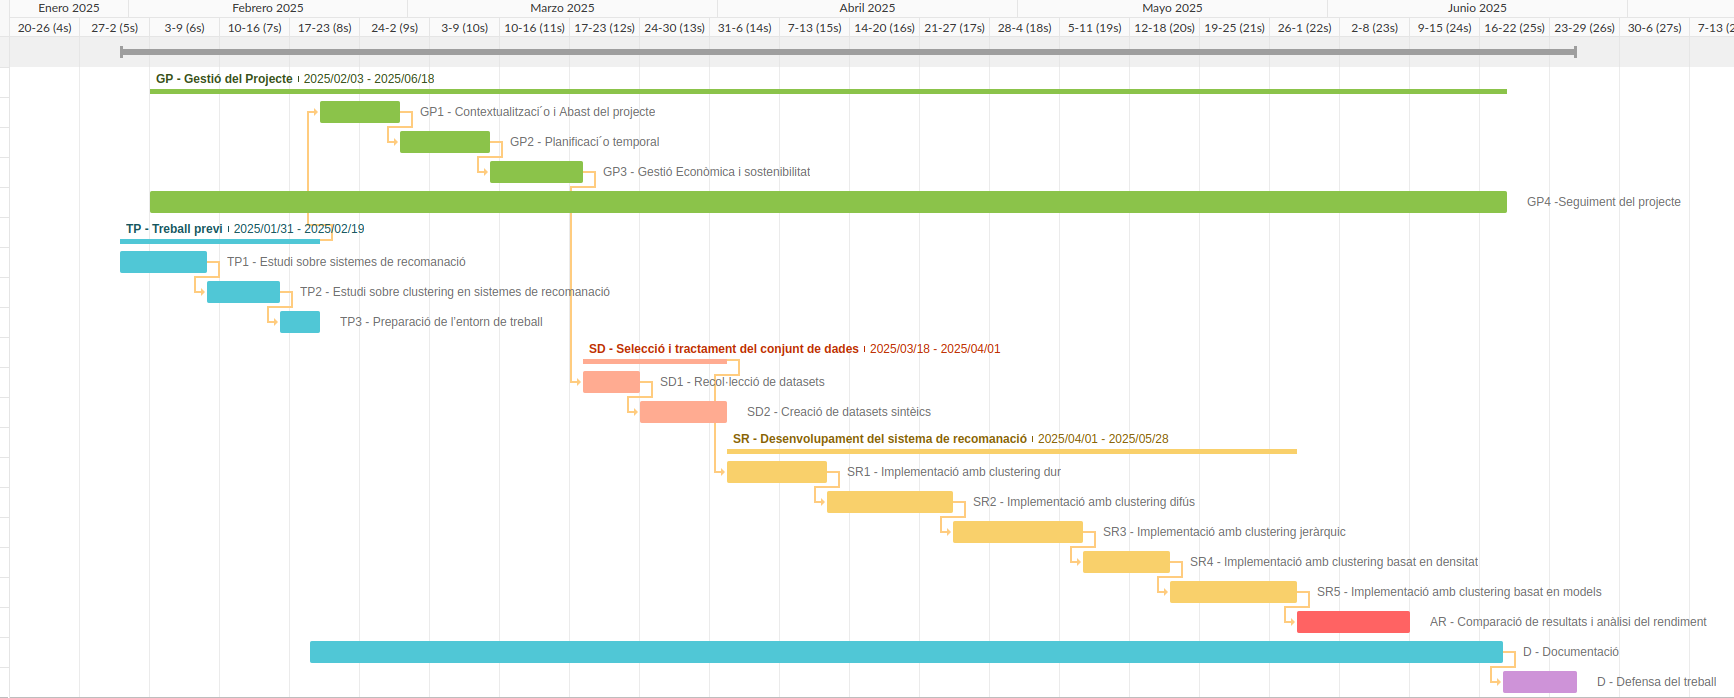
\includegraphics[width=1.5\textwidth]{Figuras/DiagramaGantt.png}
        \caption{Diagrama de Gantt creat amb GanttPro \cite{GanttPRO}}
        \label{fig:gantt}
    \end{figure}

\end{landscape} % Tornar a la orientació vertical

\section{Gestió del risc}

Tots els projectes impliquen certs riscos que cal avaluar per garantir una cobertura eficient.
La gestió de riscos és un element clau en qualsevol iniciativa, ja que permet identificar, analitzar i classificar els riscos per reduir-ne els possibles efectes negatius.
En aquest sentit, es detallen els principals riscos que podrien afectar el projecte i les estratègies de mitigació.
A la taula \ref{tab:riscos} es resumeix la probabilitat d'ocurrència i una valoració qualitativa sobre com cada risc podria influir en el desenvolupament del projecte.

\begin{table}[H]
    \centering
    \begin{tabular}{|l|c|c|}
    \hline
    \textbf{Risc}              & \textbf{Probabilitat} & \textbf{Impacte} \\ \hline
    Falta de coneixement       & Alta                  & Mitjà            \\ \hline
    Retards en la planificació & Mitjana               & Elevat           \\ \hline
    Dificultats tècniques      & Alta                  & Mitjà            \\ \hline
    Problemes amb els equips   & Baixa                 & Elevat           \\ \hline
    Complexitat computacional  & Mitjana               & Mitjà            \\ \hline
    \end{tabular}
    \caption{Taula de riscos del projecte}
    \label{tab:riscos}
\end{table}

\begin{itemize}
    \item \textbf{Falta de coneixement:} Aquest risc fa referència a la manca de coneixements previs en sistemes de recomanació i clustering, que podria dificultar el desenvolupament del projecte.
    Per mitigar aquest risc, s'ha reservat temps per a la recerca bibliogràfica i l'aprenentatge de les tècniques necessàries durant la planificació del projecte.
    \item \textbf{Retards en la planificació:} Aquest risc es refereix a la possibilitat que les tasques no s'executin segons el calendari establert, provocant endarreriments en la finalització del projecte.
    Per evitar aquest risc, es programaran reunions de seguiment periòdiques per avaluar l'estat d'execució de les tasques, es revisarà periòdicament el diagrama de Gantt i es reservaran marges temporals per absorbir possibles retards.
    \item \textbf{Dificultats tècniques:} En desenvolupar codi, és molt probable que sorgeixin imprevistos, com ara errors inesperats, incompatibilitats de llibreries o problemes de rendiment.
    Per resoldre aquests problemes, es reservarà temps extra per al desenvolupament de cada tècnica.
    \item \textbf{Problemes amb els equips:} Aquest risc contempla la possibilitat de fallades o inestabilitat en el maquinari utilitzat durant el desenvolupament i els experiments.
    Si fos necessari, es disposarà d'equips de recanvi per minimitzar la interrupció de la feina.
    \item \textbf{Complexitat computacional:} Algunes tècniques de clustering, especialment aquelles basades en models o clustering difús, poden requerir un alt consum de recursos computacionals, afectant el temps d'execució i la resposta del sistema.
    Per mitigar aquest risc, es poden optimitzar les implementacions o emprar hardware més potent, sol·licitant-lo a la universitat si cal.
\end{itemize}

\chapter{Gestió Econòmica i sostenibilitat}

\section{Gestió Econòmica}

Després d'establir la planificació temporal de la iniciativa, es procedeix a l'estimació dels costos requerits per al seu desenvolupament. S'identifiquen diverses categories de despeses, incloent-hi les associades al personal, l'espai de treball i les eines i dispositius emprats. A més, per afrontar possibles contratemps i cobrir despeses no previstes, s'elabora un pla de contingència, es defineix una partida per a imprevistos i s'estableixen mecanismes per al control pressupostari.

\subsection{Costos de personal}

A partir de la planificació de tasques, es calcula el cost de personal, tenint en compte els quatre rols definits anteriorment: Cap de projecte, Investigador, Desenvolupador i Analista.
Els costos anuals s'obtenen de la web de PayScale, que ofereix informació sobre salaris en la indústria, suposant menys d'un any d'experiència. El salari anual de cada rol es divideix pel nombre d'hores anuals de treball per obtenir el cost per hora, suposant 1.760 hores en total, tenint en compte vacances i festius.
Aquestes dades es mostren a la taula \ref{tab:costos_personal}.

\begin{table}[H]
    \centering
    \begin{tabular}{|l|c|c|}
    \hline
    \textbf{Rol}     & \textbf{Cost anual} & \textbf{Cost per hora}  \\ \hline
    Cap del projecte & 46.303€\cite{ProjectManager}             & 46.303/1.760 = 26,30€/h \\ \hline
    Investigador     & 34.000€\cite{Research}             & 34.000/1.760 = 19,32€/h \\ \hline
    Desenvolupador   & 21.237€\cite{SoftwareDeveloper}             & 21.237/1.760 = 12,07€/h \\ \hline
    Analista         & 24.439€\cite{DataAnalyst}             & 24.439/1.760 = 13,89€/h \\ \hline
    \end{tabular}
    \caption{Costos de personal}
    \label{tab:costos_personal}
\end{table}

\begin{table}[H]
    \centering
    \begin{tabular}{|l|l|c|l|c|c|}
    \hline
    \textbf{ID} & \textbf{Tasca}               & \multicolumn{1}{l|}{\textbf{Temps (h)}} & \textbf{Rols}       & \multicolumn{1}{l|}{\textbf{Cost (€)}} & \multicolumn{1}{l|}{\textbf{Cost SS (€)}} \\ \hline
    \textbf{GP} & \textbf{Gestió del Projecte} & \textbf{65}                             & \textbf{-}          & \textbf{1541,4}                        & \textbf{2003,82}                          \\ \hline
    GP1         & Contextualització            & 15                                      & J                   & 394,5                                  & 512,85                                    \\
    GP2         & Planificació temporal        & 15                                      & J                   & 394,5                                  & 512,85                                    \\
    GP3         & Sostenibilitat               & 15                                      & J                   & 394,5                                  & 512,85                                    \\
    GP4         & Seguiment del projecte       & 20                                      & J, I, D, A          & 357,9                                  & 465,27                                    \\ \hline
    \textbf{TP} & \textbf{Treball Previ}       & \textbf{55}                             & \textbf{-}          & \textbf{1062,6}                        & \textbf{1381,38}                          \\ \hline
    TP1         & Sis. de recomanació          & 25                                      & I                   & 483                                    & 627,9                                     \\
    TP2         & Clustering                   & 25                                      & I                   & 483                                    & 627,9                                     \\
    TP3         & Entorn de treball            & 5                                       & I                   & 96,6                                   & 125,58                                    \\ \hline
    \textbf{SD} & \textbf{Selecció dades}      & \textbf{40}                             & \textbf{-}          & \textbf{555,6}                         & \textbf{722,28}                           \\ \hline
    SD1         & Recol·lecció de datasets     & 15                                      & A                   & 208,35                                 & 270,855                                   \\
    SD2         & Creació de datasets          & 25                                      & A                   & 347,25                                 & 451,425                                   \\ \hline
    \textbf{SR} & \textbf{Sis. de recomanació} & \textbf{175}                            & \textbf{-}          & \textbf{2112,25}                       & \textbf{2745,925}                         \\ \hline
    SR1         & Clustering dur               & 30                                      & D                   & 362,1                                  & 470,73                                    \\
    SR2         & Clustering difús             & 40                                      & D                   & 482,8                                  & 627,64                                    \\
    SR3         & Clustering jeràrquic         & 40                                      & D                   & 482,8                                  & 627,64                                    \\
    SR4         & Clustering densitat          & 25                                      & D                   & 301,75                                 & 392,275                                   \\
    SR5         & Clustering models            & 40                                      & D                   & 482,8                                  & 627,64                                    \\ \hline
    \textbf{AR} & \textbf{Anàlisi resultats}   & \textbf{40}                             & \textbf{A}          & \textbf{555,6}                         & \textbf{722,28}                           \\ \hline
    \textbf{D}  & \textbf{Documentació}        & \textbf{60}                             & \textbf{J, I, D, A} & \textbf{1073,7}                        & \textbf{1395,81}                          \\ \hline
    \textbf{DT} & \textbf{Defensa del treball} & \textbf{15}                             & \textbf{J}          & \textbf{394,5}                         & \textbf{512,85}                           \\ \hline
    \textbf{-}  & \textbf{Total}               & \textbf{450}                            & \textbf{-}          & \textbf{7295,65}                       & \textbf{9484,345}                         \\ \hline
    \end{tabular}
    \caption[Costos de personal per tasca] {Costos de personal per tasca. 
    
    Llegenda de rols: J - Cap del projecte, I - Investigador, D - Desenvolupador, A - Analista}
    \label{tab:costos_personal_tasques}
\end{table}

A la taula \ref{tab:costos_personal_tasques} es mostren els costos de personal per tasca, on s'ha calculat el cost total de cada tasca en funció dels rols que hi intervenen i el temps que hi dediquen. En les tasques on el rol que la realitzi podria ser qualsevol, s'ha suposat el cost mitjà per hora dels rols.

El cost total de personal és de 7.295,65 €, mentre que el cost total de personal amb seguretat social, suposant un 30 \%, és de 9.484,35 €.

\subsection{Costos genèrics}

Tot el software utilitzat en el projecte és de codi obert, per tant, no hi ha cap cost associat a l'adquisició de llicències. El cost total de software és de 0 €.

Per realitzar el projecte, s'utilitza un ordinador portàtil ASUS amb un preu de 699€. Es calcula l'amortització tenint en compte que a l'any hi ha 220 dies laborables i 8 hores laborables al dia, segons la següent fórmula:

Es considera una vida útil de 5 anys.

\begin{equation}
    \text{Amortització} = \frac{\text{Preu ordinador}}{\text{Dies laborables} \times \text{Hores laborables} \times \text{Vida útil}} \times \text{Hores d'ús}
\end{equation}

\begin{equation}
    \text{Amortització} = \frac{699}{220 \times 8 \times 5} \times 450 = 35,74 \text{€}
\end{equation}

El projecte també té associats una sèrie de costos indirectes:

\begin{itemize}
    \item L'electricitat té un cost mitjà de 0,215€/kWh. El portàtil té un consum de 45W. Suposant que el portàtil estarà encès 430 hores, el cost de l'electricitat és de 0,215€/kWh * 0,045kW * 430h = 4,16€.
    \item Internet té un cost de 40€/mes. Suposant que el projecte duri 5 mesos, el cost total és de 40€/mes * 5 mesos = 200€.
    \item El desplaçament per a reunions de seguiment i altres té un cost de 44€ de manera trimestral, així que el cost total és de 44€ * 2 = 88€.
    \item El projecte es desenvolupa íntegrament a l'habitatge propi de l'autor, però si hagués de llogar l'habitació, el preu aproximat seria de 400€/mes. Suposant que el projecte duri 5 mesos, el cost total és de 400€/mes * 5 mesos = 2000€.
\end{itemize}

A la taula \ref{tab:costos_generics} es mostra un resum dels costos genèrics del projecte. El cost total de costos genèrics és de 2.277,9 €.

\begin{table}[H]
    \centering
    \begin{tabular}{|l|c|}
    \hline
    \textbf{Concepte} & \textbf{Cost (€)} \\ \hline
    Amortització      & 35,74             \\
    Electricitat      & 4,16              \\
    Internet          & 150               \\
    Desplaçament      & 88                \\ 
    Lloc de treball   & 2000              \\ \hline
    \textbf{Total}    & \textbf{2277,9}  \\ \hline
    \end{tabular}
    \caption{Costos genèrics}
    \label{tab:costos_generics}
\end{table}

\subsection{Contingències}

En qualsevol iniciativa, és essencial incorporar un marge addicional per afrontar possibles contratemps i imprevistos. En aquest context, atès que es tracta d’un estudi basat en tecnologies emergents, hi ha una alta probabilitat d’enfrontar-se a desafiaments durant la seva execució. Per això, s’ha determinat establir un marge del 15 \% per cobrir aquests costos addicionals.

El cost de contingència es calcula amb la fórmula següent:

\begin{equation}
    \text{Cost contingència} = (\text{Cost total de personal} + \text{Cost total genèric}) \times 0,15
\end{equation}

\begin{equation}
    \text{Cost contingència} = (9484,35 + 2277,9) \times 0,15 = 1764,34 \text{€}
\end{equation}

\subsection{Imprevistos}

És fonamental tenir en compte les despeses derivades dels eventuals contratemps que puguin sorgir al llarg de l’execució d’aquest projecte. Com s’ha indicat prèviament, és important establir mesures per mitigar els possibles riscos associats a la realització de la tasca.

Per determinar el cost dels imprevistos, s’aplica la fórmula següent:

\begin{equation}
    \text{Cost imprevist} = \text{Cost} \times \frac{\text{Probabilitat (\%)}}{100}
\end{equation}

\begin{table}[H]
    \centering
    \begin{tabular}{|l|c|c|c|c|}
    \hline
    \textbf{Imprevist}               & \textbf{Cost (€)} & \textbf{Prob. (\%)} & \textbf{Rol} & \textbf{Cost imprevist (€)} \\ \hline
    Increment desenvolupament (25 h) & 392,275           & 20                  & D            & 78,455                      \\
    Nou portàtil                     & 699               & 5                   & -            & 34,95                       \\ \hline
    \textbf{Total}                   & \textbf{-}        & \textbf{-}          & \textbf{-}   & \textbf{113,405}            \\ \hline
    \end{tabular}
    \caption[Costos imprevistos] {Costos imprevistos.

    Llegenda de rols: D - Desenvolupador}
    \label{tab:costos_imprevistos}
\end{table}

A la taula \ref{tab:costos_imprevistos} es mostren els costos dels imprevistos, on s'ha calculat el cost total de cada imprevist en funció de la probabilitat que succeeixi.

El risc de necessitar més temps de desenvolupament és alt, per la qual cosa s'estima una probabilitat del 20\% i un cost de 25 hores de desenvolupament. El risc de necessitar un nou portàtil és baix, per la qual cosa s'estima una probabilitat del 5\% i el cost d'un portàtil.

\subsection{Cost total}

A continuació es presenta una taula resum \ref{tab:cost_total} amb el cost total del projecte. El cost total del projecte és de 13.639,99 €.

\begin{table}[H]
    \centering
    \begin{tabular}{|l|c|}
    \hline
    \textbf{Tipus}       & \textbf{Cost}     \\ \hline
    Cost personal        & 9484,345          \\
    Cost genèrics        & 2277,9            \\
    Cost de contingència & 1764,34           \\
    Cost imprevistos     & 113,405           \\ \hline
    \textbf{Cost total}  & \textbf{13639,99} \\ \hline
    \end{tabular}
    \caption{Cost total del projecte}
    \label{tab:cost_total}
\end{table}

\subsection{Control de gestió}

El control de gestió té com a objectiu principal supervisar, avaluar i ajustar de manera contínua totes les operacions del projecte per tal d’assegurar el compliment dels objectius establerts. Per aconseguir-ho, és imprescindible definir indicadors quantitatius que permetin mesurar el rendiment i detectar desviacions respecte al pressupost, el cronograma i els recursos planificats.

A continuació, es presenten alguns dels indicadors i mètriques que s’utilitzaran:

\begin{enumerate}
    \item Desviació cost personal per tasca:
    \[
    (\text{cost\_estimat} - \text{cost\_real}) * \text{hores\_reals}
    \]

    \item Desviació realització tasques:
    \[
    (\text{hores\_estimades} - \text{hores\_reals}) * \text{cost\_real}
    \]

    \item Desviació total realització tasca:
    \[
    \text{cost\_estimat} - \text{cost\_real}
    \]

    \item Desviació cost genèric:
    \[
    \text{cost\_estimat\_genèric} - \text{cost\_real\_genèric}
    \]

    \item Desviació cost imprevistos:
    \[
    \text{cost\_imprevistos\_estimat} - \text{cost\_imprevistos\_real}
    \]

    \item Desviació hores del projecte:
    \[
    \text{hores\_estimades} - \text{hores\_reals}
    \]

\end{enumerate}

Aquest control es durà a terme de manera periòdica mitjançant reunions bisetmanals, on es revisaran i actualitzaran els indicadors mitjançant una fulla de càlcul. En acabar cada tasca, es compararan les dades reals amb les estimades. A més, es registraran de forma detallada tots els despeses extra derivats d’imprevistos i contingències, de manera que qualsevol desviació, especialment aquella superior al 5\, pugui ser identificada i corregida a temps.

En cas de detectar desviacions negatives (per exemple, un cost superior al previst o retards en el cronograma), es prendran mesures correctives com ara:

\begin{itemize}
    \item Augmentar el pressupost mitjançant el fons reservat per a contingències.
    \item Ajustar el temps assignat o reassignar tasques per optimitzar el consum d’hores.
    \item Reduir o modificar parts del projecte per minimitzar els efectes dels desajustos detectats.
\end{itemize}

Aquest enfocament proactiu permetrà no només identificar ràpidament qualsevol desviació, sinó també actuar de manera eficaç per mantenir el projecte dins dels paràmetres planificats i assegurar-ne l’èxit global.

\section{Sostenibilitat}

Al llarg dels meus estudis en el Grau d'Enginyeria Informàtica a la FIB, he tingut l'oportunitat d'aprofundir en els aspectes clau de la sostenibilitat a través de diverses assignatures, reconeixent la seva importància durant el desenvolupament del TFG.

La sostenibilitat, entesa des d'una perspectiva integral que inclou les dimensions econòmica, social i ambiental, és un factor essencial en qualsevol projecte, tant si és de gran com de petita escala. A nivell personal, sempre he considerat fonamental l'anàlisi econòmica per garantir la viabilitat d'un projecte, ja que sovint es busca millorar l'eficiència econòmica d'una solució existent.

A més, aquest treball m'ha permès reflexionar sobre la importància d'abordar la sostenibilitat de manera global. He observat que, en moltes ocasions, es dona més pes als beneficis econòmics en detriment de les dimensions social i ambiental, un fet que considero crucial per assolir un impacte positiu i sostenible en el temps.

Finalment, crec que tots els projectes s'haurien de desenvolupar amb l'objectiu de cobrir una necessitat real de la societat.

\subsection{Dimensió econòmica}

El projecte s'ha plantejat amb una acurada estimació de costos, on s'han identificat i analitzat de manera detallada les diferents parts de personal, despeses genèriques, contingències i imprevistos. Així, en el PPP s'estableix un pressupost realista (aproximadament 13.640 €) que permet debatre tant la viabilitat econòmica del projecte com l'adequada assignació de recursos.

Pel que fa a la vida útil i a la resolució actual dels aspectes de costos del problema, l’estat de l’art aposta pel ús de tecnologies de codi obert i models d’anàlisi que optimitzen la gestió de dades. No obstant això, moltes de les solucions vigents no aborden completament el repte del cost computacional derivat del processament de grans volums de dades, aspecte que es compensa en el nostre enfocament mitjançant l’aplicació de tècniques de clustering que redueixen la dispersió i milloren l’eficiència.

Finalment, la solució proposada ofereix una millora econòmica significativa en comparació amb els mètodes existents. En incorporar el clustering com a pas previ al filtratge col·laboratiu, s’optimitzen els temps de processament i es redueix el consum de recursos computacionals, cosa que es tradueix en menys costos operatius i en una major rendibilitat i sostenibilitat a llarg termini.

\subsection{Dimensió ambiental}

Atès que es tracta d’un projecte de recerca i investigació dels diferents mètodes de clustering en sistemes recomanadors, l’impacte ambiental associat prové principalment del consum d’electricitat, sobretot si aquesta electricitat es genera a partir de fonts d’energia no renovables. El càlcul del consum elèctric que s'ha determinat correspon a l’electricitat consumida pel portàtil.

Al reutilitzar el portàtil, s’evita la producció de residus electrònics i es redueix l’impacte ambiental associat a la fabricació de nous dispositius. A més, la durada de vida útil del portàtil es veu ampliada gràcies a la seva correcta gestió i manteniment, la qual cosa contribueix a minimitzar el consum de recursos naturals i a reduir l’emissió de gasos contaminants.

En l’estat de l’art actual les solucions aborden el problema principal des d’un punt de vista tecnològic, però sovint no integren de manera completa criteris ambientals. La nostra proposta millora ambientalment les solucions existents, ja que no només optimitza els processos i redueix el consum de recursos, sinó que també incorpora mesures específiques per disminuir l’emissió de residus i l’ús energètic, contribuint així a una reducció global de l’impacte ambiental.

\subsection{Dimensió social}

La realització del projecte posat en producció suposa, a nivell personal, una gran oportunitat per créixer tant professionalment com humanament. A més d’ampliar els meus coneixements en àrees com la intel·ligència artificial i l’anàlisi de dades, em permetrà desenvolupar habilitats en la gestió i coordinació de projectes reals, fet que enriquirà el meu perfil professional.

D’altra banda, actualment el problema que es vol abordar es resol amb sistemes de recomanació basats en mètodes tradicionals, com el filtratge col·laboratiu, que tot i ser útils, presenten limitacions pel que fa a la personalització i l’eficiència. La solució que proposo pretén millorar socialment la qualitat de vida dels usuaris, oferint recomanacions més ajustades a les seves necessitats i interessos, fet que afavoreix una interacció més rellevant i satisfactòria.

inalment, existeix una necessitat real d’aquest projecte, ja que l’increment exponencial de la informació digital exigeix noves eines que superin les limitacions dels mètodes actuals. Això no sols permetrà una millor gestió dels recursos, sinó que també contribuirà a millorar la qualitat de vida social a través d’una experiència d’usuari més adaptada i eficient.

\printbibliography[heading=bibintoc]

\restoregeometry % Restaurar la configuració de marges original si és necessari

\end{document}